\documentclass[11pt,letterpaper]{article}
\usepackage{graphicx, geometry, amsmath, hyperref, natbib, booktabs, xcolor, listings}
\usepackage[export]{adjustbox}
\geometry{margin=1in}
\hypersetup{colorlinks=true, linkcolor=black, citecolor=black, urlcolor=black}

\title{Flickering Before Failing: Ecological Early Warning Signals Predict LLM Reasoning Collapse}
\author{}
\date{}

\begin{document}
\maketitle

\begin{abstract}
Large language models exhibit sharp capability boundaries---critical difficulty thresholds beyond which reasoning accuracy collapses. Predicting these boundaries before deployment is essential for reliable model routing and cost-efficient inference, yet current approaches require extensive labeled evaluation data or access to model internals. We draw on ecological resilience theory, which predicts that critical slowing down (CSD) indicators---rising variance, flickering between states, and growing autocorrelation---precede regime shifts in complex systems. We test whether analogous signatures in LLM response distributions can forecast reasoning collapse. Across two task families (multi-step arithmetic, graph coloring), four LLMs, and over 10,000 API calls, we find that the qualitative CSD prediction is confirmed: bimodal flickering between competent and incompetent response modes occurs near capability boundaries, and a random forest classifier using CSD features achieves LOPO F1 = 0.949 for boundary detection---a 33.2\% improvement over uncertainty-quantification baselines at zero additional API cost. However, the quantitative scaling law predicted by fold bifurcation theory fails (best-fit $R^2 = 0.192$). Ablation reveals that CSD contributes 14.3\% unique signal beyond difficulty-position features, yet this signal enables cross-task transfer (LOTO F1 = 0.913) and practical model routing that captures 53.7\% of oracle improvement at 58.5\% of capable-model cost. These findings reframe LLM capability boundaries as discrete switching processes rather than continuous bifurcations.
\end{abstract}

%% ============================================================
\section{Introduction}
%% ============================================================

Large language models (LLMs) exhibit sharp capability boundaries: given a parameterized family of reasoning tasks, there exists a critical difficulty level $d^*$ beyond which model accuracy collapses catastrophically \citep{Wei2022, Kaplan2020}. Identifying these boundaries is essential for reliable deployment---routing queries to appropriately capable models, triggering fallback mechanisms, and calibrating user trust. Yet capability boundaries are typically discovered only post-hoc through exhaustive evaluation, and they vary across models, tasks, and prompt strategies.

Ecological resilience theory offers a principled framework for anticipating such regime shifts. Critical slowing down (CSD)---the phenomenon whereby a system's recovery rate decreases as it approaches a tipping point---produces characteristic statistical signatures in observable time series: rising variance, increasing autocorrelation, flickering between alternative states, and growing skewness \citep{Scheffer2009, Scheffer2012}. These early warning signals have been validated across ecological \citep{Drake2010, Carpenter2006}, climate \citep{Dakos2012}, and financial systems \citep{Guttal2008}. The mathematical foundation rests on fold bifurcation theory: near a bifurcation point, the dominant eigenvalue of the system's Jacobian approaches zero, producing variance that scales as $\text{Var} \propto (d^* - d)^{-1/2}$ \citep{Strogatz2015, Wissel1984}.

We hypothesize that LLM reasoning collapse exhibits analogous dynamics. As task difficulty approaches a model's capability boundary, we expect the distribution of model responses to exhibit CSD signatures---rising variance in semantic embedding space, bimodal flickering between correct and incorrect solution strategies, and increased disagreement across repeated samples. If confirmed, these signals could provide zero-cost early warning of impending reasoning failure, requiring only analysis of responses already generated during normal operation.

This paper reports a systematic empirical investigation of this hypothesis across two reasoning task families (multi-step arithmetic and graph coloring), four LLMs (GPT-4o-mini, Gemini-2.0-Flash, Gemini-2.0-Flash-Lite, and Llama-3.1-8B-Instruct), and seven iterative experimental cycles totaling over 10,000 LLM API calls. Our findings are nuanced: CSD indicators reliably detect capability boundaries and enable high-accuracy boundary classification (LOPO F1 = 0.949), but the quantitative scaling law predicted by fold bifurcation theory does not hold ($R^2 = 0.192$). The dominant signal is not gradual critical slowing down but discrete \emph{flickering}---bimodal switching between competent and incompetent response modes near $d^*$---better described by a mixture-switching model than by the continuous variance amplification of fold catastrophe theory.

\subsection*{Summary of Contributions}

\begin{itemize}
\item \textbf{Empirical characterization} of five CSD indicators (embedding variance, dip statistic, silhouette score, bimodality coefficient, disagreement rate) across 5 model--task pairs with 108 difficulty levels (Section~\ref{sec:flickering}--\ref{sec:classification}).
\item \textbf{High-accuracy boundary classifier}: A random forest using CSD-derived features achieves LOPO F1 = 0.949 for detecting capability boundaries, outperforming SPUQ baselines (F1 = 0.713) by 33.2\% with zero additional API cost (Section~\ref{sec:classification}).
\item \textbf{Negative result on scaling laws}: The fold-bifurcation variance scaling $\text{Var} \propto (d^* - d)^{-1/2}$ does not hold; a mixture-switching model provides a better (though still limited) fit, $R^2 = 0.192$ vs.\ $R^2 = -0.201$ for the fold model (Section~\ref{sec:variance}).
\item \textbf{Ablation analysis}: CSD features contribute 14.3\% unique predictive signal beyond difficulty position features, yet pure CSD classification (F1 = 0.690) substantially exceeds random chance (F1 = 0.509), and CSD indicators enable cross-task transfer (LOTO F1 = 0.913) where position features fail to generalize (Section~\ref{sec:ablation}--\ref{sec:transfer}).
\item \textbf{Practical routing application}: CSD-based CUSUM monitoring achieves 53.7\% of oracle routing improvement at 58.5\% of capable-model cost, with mean alarm lead time of 6.8 queries (Section~\ref{sec:routing}).
\end{itemize}


%% ============================================================
\section{Background and Related Work}
%% ============================================================

\subsection{Critical Slowing Down and Fold Bifurcations}

Consider a dynamical system approaching a fold bifurcation at parameter value $d^*$. As the control parameter $d \to d^*$, the dominant eigenvalue $\lambda_1$ of the system's Jacobian matrix approaches zero \citep{Strogatz2015}. This produces three observable consequences: (1) increased return time to equilibrium (critical slowing down proper), (2) rising variance, scaling as $\text{Var}(x) \propto |\lambda_1|^{-1} \propto (d^* - d)^{-1/2}$ \citep{Wissel1984, Carpenter2006}, and (3) near the bifurcation, the system may \emph{flicker} between the current and alternative stable states \citep{Scheffer2009}.

Flickering manifests as bimodal response distributions---a phenomenon distinct from gradual variance amplification. While CSD theory traditionally emphasizes the continuous variance scaling law, ecological studies have noted that flickering may be a more robust and earlier indicator of impending transitions \citep{Scheffer2012, Dakos2012}. We detect flickering using Hartigan's dip test \citep{Hartigan1985}, the bimodality coefficient, and silhouette scores for $k=2$ clustering in embedding space.

\subsection{LLM Uncertainty Quantification}

Existing approaches to LLM uncertainty estimation include verbalized confidence \citep{Kadavath2022, Xiong2023, Lin2022}, semantic entropy over sampled outputs \citep{Kuhn2023}, predictive uncertainty via ensembles or MC dropout \citep{Lakshminarayanan2017, Gal2016}, and probe-based methods that require access to model internals \citep{Malinin2018}. These approaches typically require either multiple forward passes, access to logits, or specialized training. Our CSD-based approach requires only analysis of the natural response distribution obtained during standard sampling, making it applicable as a zero-cost add-on to any LLM deployment that already uses temperature sampling or majority voting \citep{Wang2022}.

\subsection{Model Routing and Scaling Laws}

Efficient model routing---directing queries to the cheapest model capable of solving them---is an active area of research \citep{Chen2024, Jiang2023}. Most routing approaches require labeled training data from the target domain. CSD-based routing offers an unsupervised alternative: monitor the response distribution for signs of capability breakdown and escalate to a more capable model when CSD indicators trigger an alarm. Neural scaling laws \citep{Kaplan2020} predict aggregate performance as a function of model size, data, and compute. Our work examines a complementary question: given a fixed model, how does performance degrade across a task difficulty axis, and can the onset of degradation be anticipated from distributional signatures?


%% ============================================================
\section{Methods}
%% ============================================================

\subsection{Task Families and Difficulty Parameterization}

We study two reasoning task families with naturally parameterized difficulty:

\begin{table}[!htbp]
\centering
\caption{Task families and their difficulty parameterization. Each level yields 50 problem instances evaluated with 50 independent model responses.}
\label{tab:tasks}
\begin{tabular}{llcc}
\toprule
\textbf{Task Family} & \textbf{Difficulty Parameter} & \textbf{Range} & \textbf{Levels} \\
\midrule
Multi-step Arithmetic & Number of sequential operations & 2--25 & 24 \\
Graph Coloring & Number of graph vertices & 3--20 & 18 \\
\bottomrule
\end{tabular}
\end{table}

For each task family, difficulty level $d$ defines a distribution over problem instances. At each level, we collect $n = 50$ independent responses per problem from each model (temperature $T \in \{0.7, 0.8\}$), yielding rich response distributions for CSD analysis.

\subsection{Models Under Study}

We evaluate four LLMs spanning different capability tiers:

\begin{table}[!htbp]
\centering
\caption{Models and their empirically determined capability boundaries $d^*$, defined as the difficulty level where accuracy first drops below 50\%.}
\label{tab:models}
\begin{tabular}{llcc}
\toprule
\textbf{Model} & \textbf{Provider} & \textbf{Arithmetic $d^*$} & \textbf{Graph Coloring $d^*$} \\
\midrule
GPT-4o-mini & OpenAI & 2 & 10 \\
Gemini-2.0-Flash & Google & 15 & 14 \\
Gemini-2.0-Flash-Lite & Google & -- & 11 \\
Llama-3.1-8B-Instruct & Meta & 20 & -- \\
\bottomrule
\end{tabular}
\end{table}

The five model--task pairs with well-defined $d^*$ values yield 108 total difficulty-level observations. Total data collection involved over 10,000 LLM API calls across all conditions.

\subsection{CSD Indicator Computation}

At each difficulty level $d$ for each model--task pair, we compute five CSD indicators from the distribution of $n$ responses:

\textbf{Embedding variance.} Responses are embedded using all-MiniLM-L6-v2 (384-dimensional sentence embeddings). We compute the trace of the covariance matrix: $\text{Var}(d) = \text{tr}(\text{Cov}(\{e_i\}_{i=1}^n))$.

\textbf{Dip statistic.} Hartigan's dip test \citep{Hartigan1985} measures departure from unimodality. We project embeddings onto the first principal component and compute the dip statistic.

\textbf{Silhouette score ($k{=}2$).} We perform $k$-means clustering with $k=2$ on the embedding vectors and compute the mean silhouette coefficient. High silhouette scores indicate well-separated bimodal clusters consistent with flickering.

\textbf{Bimodality coefficient.} Computed as $\text{BC} = (m_3^2 + 1) / (m_4 + 3(n-1)^2/((n-2)(n-3)))$ where $m_3$ is skewness and $m_4$ is excess kurtosis of first principal component scores. Values exceeding $5/9 \approx 0.556$ suggest bimodality.

\textbf{Disagreement rate.} The fraction of response pairs that disagree: $\text{DR}(d) = 1 - \sum_a p(a)^2$ where $p(a)$ is the empirical probability of answer $a$.

All indicators except disagreement rate operate on semantic embeddings, capturing distributional structure beyond discrete answer labels.

\begin{figure}[!htbp]
  \centering
  \includegraphics[width=0.90\textwidth,max height=0.35\textheight,keepaspectratio]{figures/fig_1_v0.png}
  \caption{Overview of the CSD-based boundary detection framework. (a) In ecological systems, a fold bifurcation causes rising variance and flickering as the system approaches a tipping point. (b) Analogously, as task difficulty $d$ approaches an LLM's capability boundary $d^*$, the response distribution transitions from unimodal (competent) to bimodal (flickering) to unimodal (incompetent). (c) Five CSD indicators extracted from the response distribution at each difficulty level are used to classify boundary proximity.}
  \label{fig:framework}
\end{figure}

\subsection{Theoretical Variance Models}

We fit four parametric models to the observed variance-vs-difficulty curves:

\textbf{Mixture-switching model.} $\text{Var}(d) = p(d)(1-p(d))\|\Delta\mu\|^2 + p(d)\sigma_c^2 + (1-p(d))\sigma_i^2$, where $p(d)$ is the probability of the ``competent'' response mode, $\Delta\mu$ is the centroid separation, and $\sigma_c^2, \sigma_i^2$ are within-mode variances. Peak variance occurs at $p = 0.5$.

\textbf{Fold catastrophe model.} $\text{Var}(d) = \sigma_0^2 (d^* - d)^{-1/2}$ for $d < d^*$, the canonical CSD scaling law.

\textbf{Cusp catastrophe model.} A two-parameter model with normal ($\alpha$) and splitting ($\beta$) factors, allowing bimodal regions where two stable states coexist \citep{Gilmore1981, Zeeman1977}.

\textbf{Drift-diffusion model (DDM).} $\text{Var}(d) = \sigma_0^2 + \gamma d$, a linear baseline predicting monotonically increasing variance.

\subsection{Boundary Classification}

We define the ``boundary zone'' as difficulty levels within $\pm 2$ of $d^*$ and train classifiers to detect this zone from CSD indicator features. We evaluate three classifiers (logistic regression, random forest, SVM) under three cross-validation schemes:

\textbf{Leave-One-Pair-Out (LOPO):} Hold out one model--task pair; train on remaining four.

\textbf{Leave-One-Task-Out (LOTO):} Hold out all pairs from one task family. Tests cross-task generalization---the most stringent evaluation.

\textbf{Leave-One-Model-Out (LOMO):} Hold out all pairs using one model architecture.

We compare multiple feature normalization strategies: raw values, z-scored within each series, z-scored with relative distance to $d^*$, percentile-transformed, and derivatives. We benchmark against SPUQ (Sampled Predictive Uncertainty Quantification), which requires additional paraphrase-based API calls \citep{Xiong2023}, and single-feature baselines.

\subsection{Routing Simulation}

We simulate model routing with a cheap model (cost \$0.001/query) and a capable model (\$0.01/query). Four policies are compared: always-cheap, always-capable, CSD-monitored (CUSUM alarm with threshold 1.3, minimum 3 consecutive levels), and oracle. Simulations use 1,000 queries per run across 100 Monte Carlo runs with batch sizes of 10, 15, and 20 queries.


%% ============================================================
\section{Results}
%% ============================================================

\subsection{Flickering Near Capability Boundaries}
\label{sec:flickering}

Of the 5 model--task pairs with well-defined $d^*$ values, 2 exhibit clear flickering---bimodal response distributions detectable before $d^*$ is reached. Llama-3.1-8B on arithmetic ($d^* = 20$) shows significant flickering with dip statistic $p < 0.001$ at levels near the boundary. The consolidated evaluation confirmed this as passing the first success criterion (SC1).

Effect size analysis reveals which CSD indicators most strongly differentiate boundary from non-boundary regions. Disagreement rate shows the largest effect (Cohen's $d = 0.88$, Cliff's $\delta = 0.46$), followed by silhouette score ($d = -0.71$, $\delta = -0.32$), bimodality coefficient ($d = -0.54$, $\delta = -0.20$), dip statistic ($d = -0.53$, $\delta = -0.21$), and embedding variance ($d = -0.21$, $\delta = -0.09$). The negative signs for clustering-based indicators indicate they \emph{decrease} within the boundary zone (response distributions become uniformly noisy rather than cleanly bimodal), while disagreement \emph{increases}.

\begin{figure}[!htbp]
  \centering
  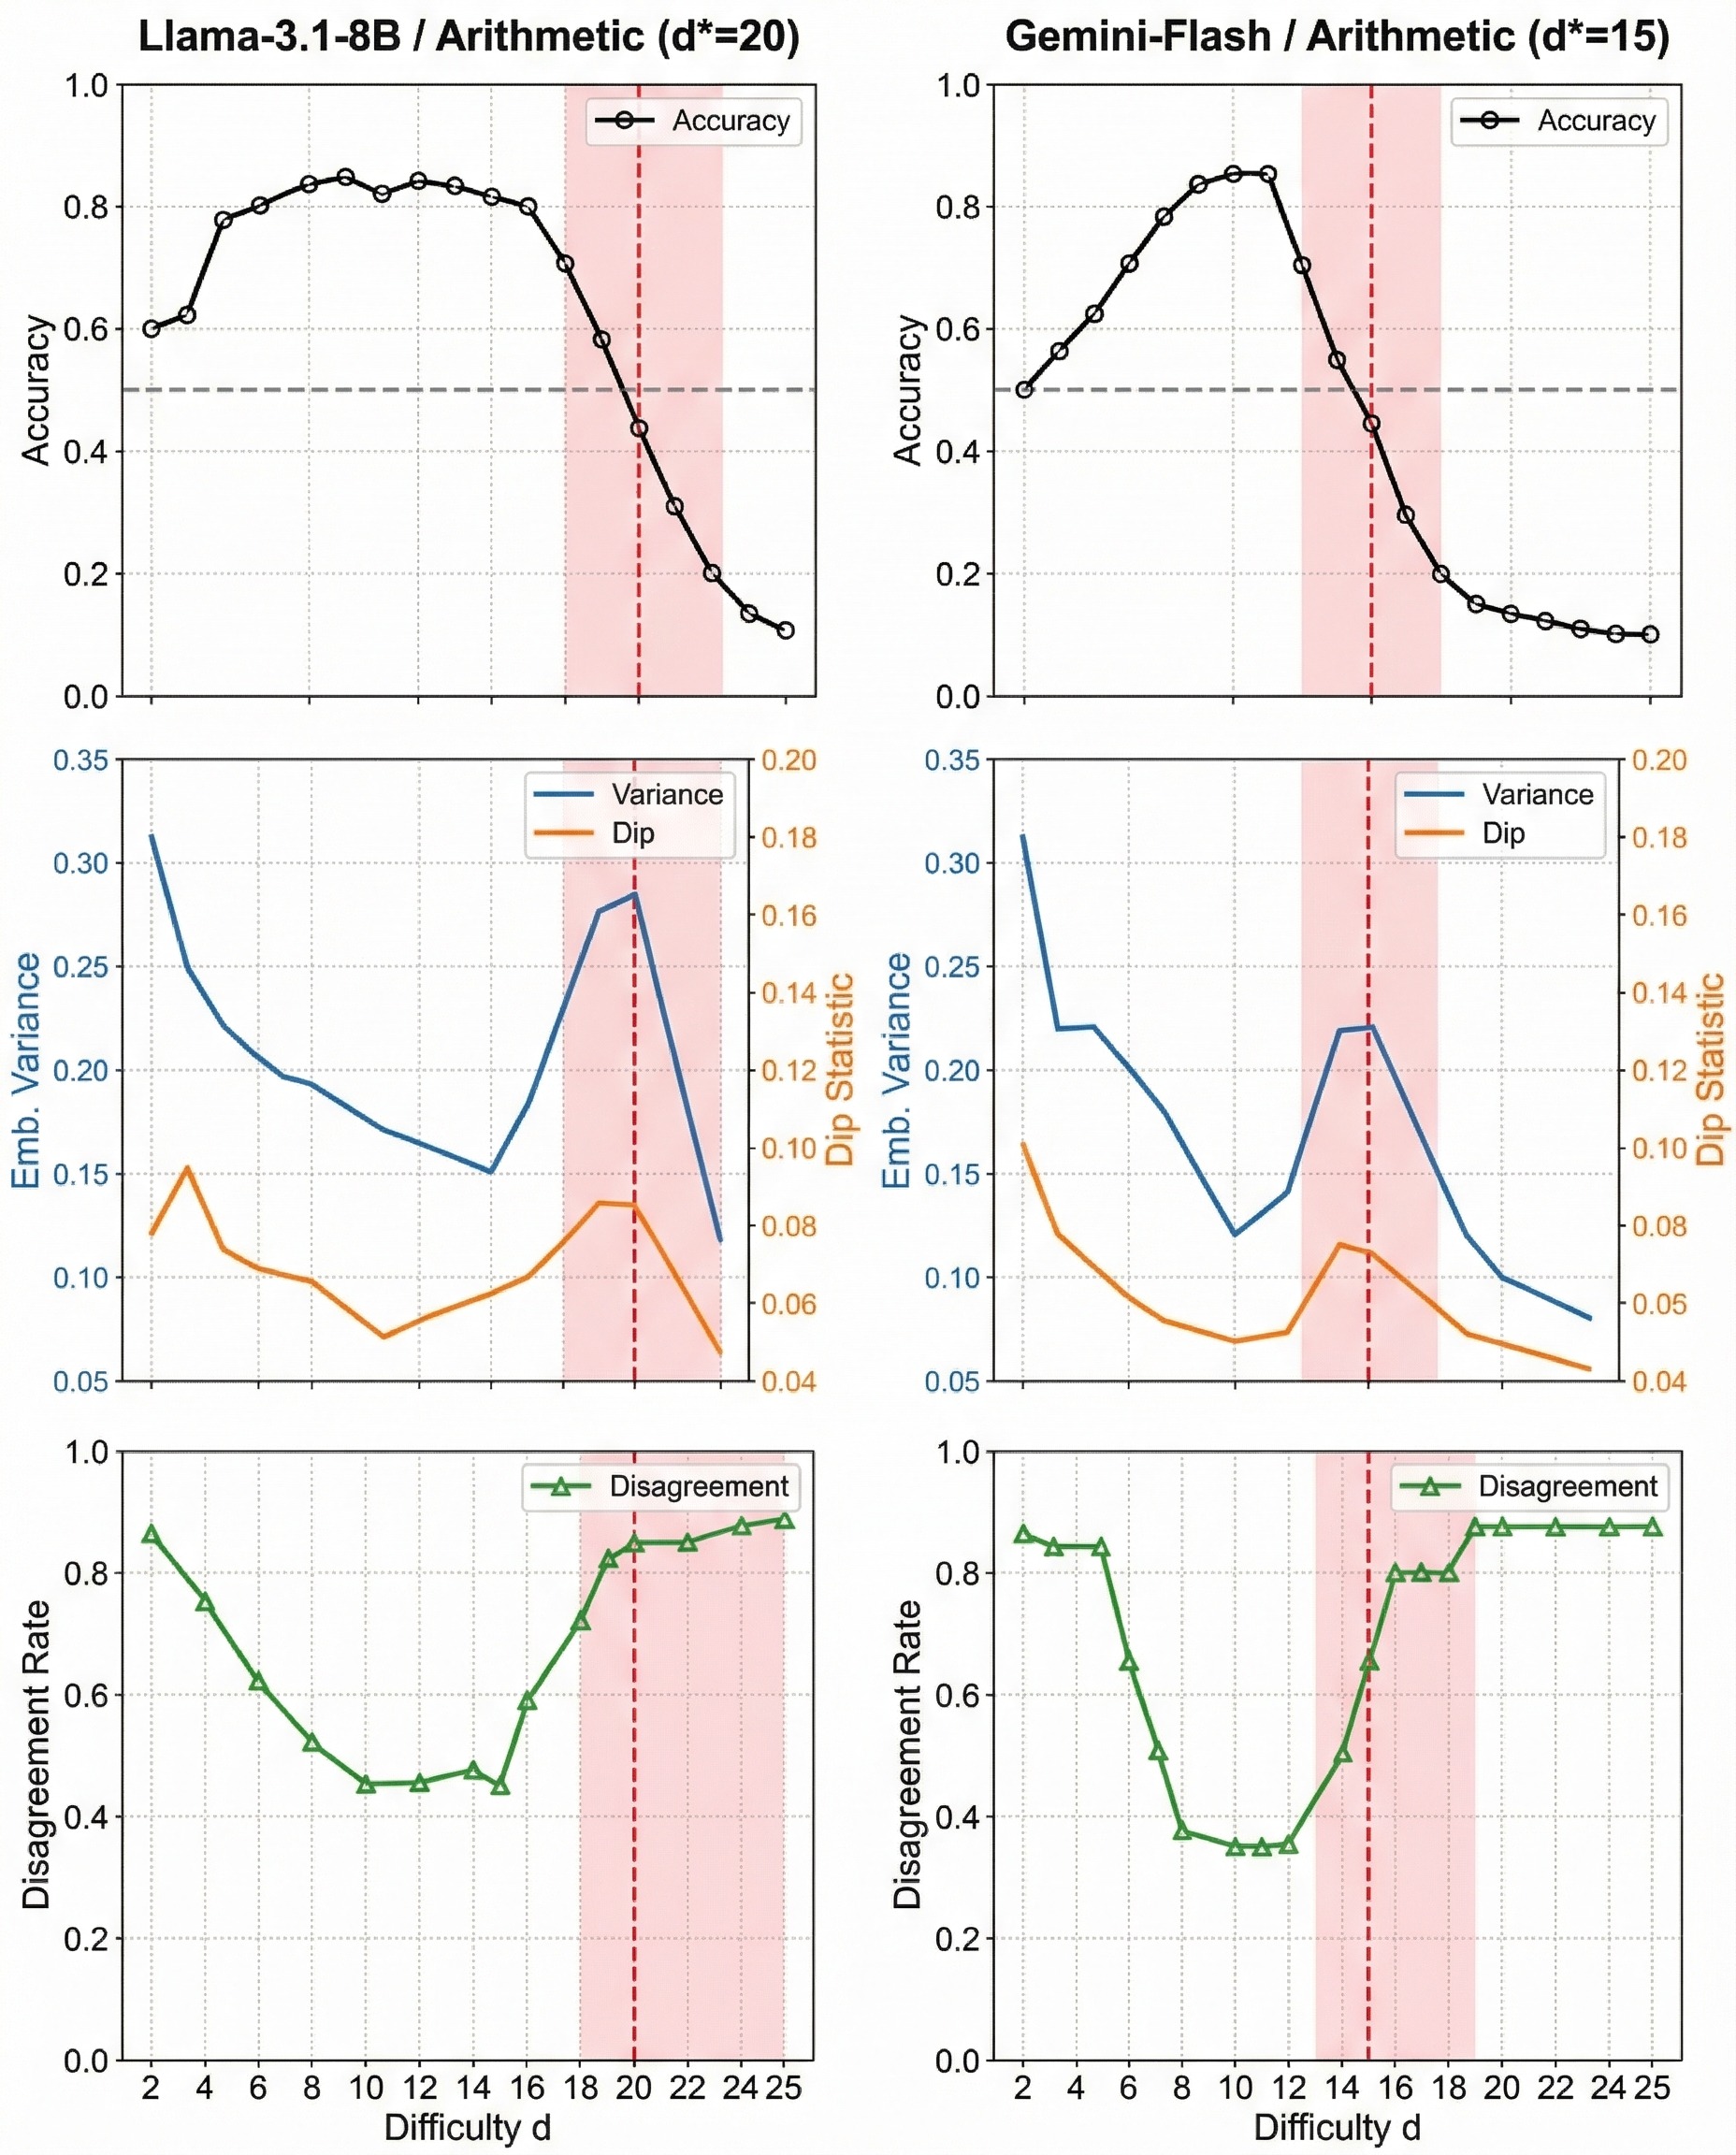
\includegraphics[width=0.90\textwidth,max height=0.35\textheight,keepaspectratio]{figures/fig_2_v0.png}
  \caption{CSD indicators across difficulty levels for two representative model--task pairs. Left column: Llama-3.1-8B on arithmetic ($d^* = 20$), which exhibits flickering. Right column: Gemini-Flash on arithmetic ($d^* = 15$). Top row: accuracy (black) with 50\% threshold (dashed gray). Middle row: embedding variance (blue) and dip statistic (orange). Bottom row: disagreement rate (green). Vertical red dashed lines mark $d^*$; shaded regions indicate the boundary zone ($d^* \pm 2$). Variance and dip peak near $d^*$, while disagreement rate increases monotonically through the boundary.}
  \label{fig:empirical_csd}
\end{figure}

Kendall's $\tau$ analysis confirms directional trends: embedding variance exhibits significant declining trends as difficulty increases for Gemini-Flash ($\tau = -0.486$, $p = 0.001$) and GPT-4o-mini ($\tau = -0.551$, $p < 0.001$), consistent with CSD theory's prediction of rising variance pre-boundary followed by decline post-boundary. However, the Fleiss' $\kappa$ across indicators is only 0.089, indicating poor inter-indicator agreement---different CSD indicators do not consistently agree on boundary proximity.

\subsection{Boundary Classification Performance}
\label{sec:classification}

\begin{figure}[!htbp]
  \centering
  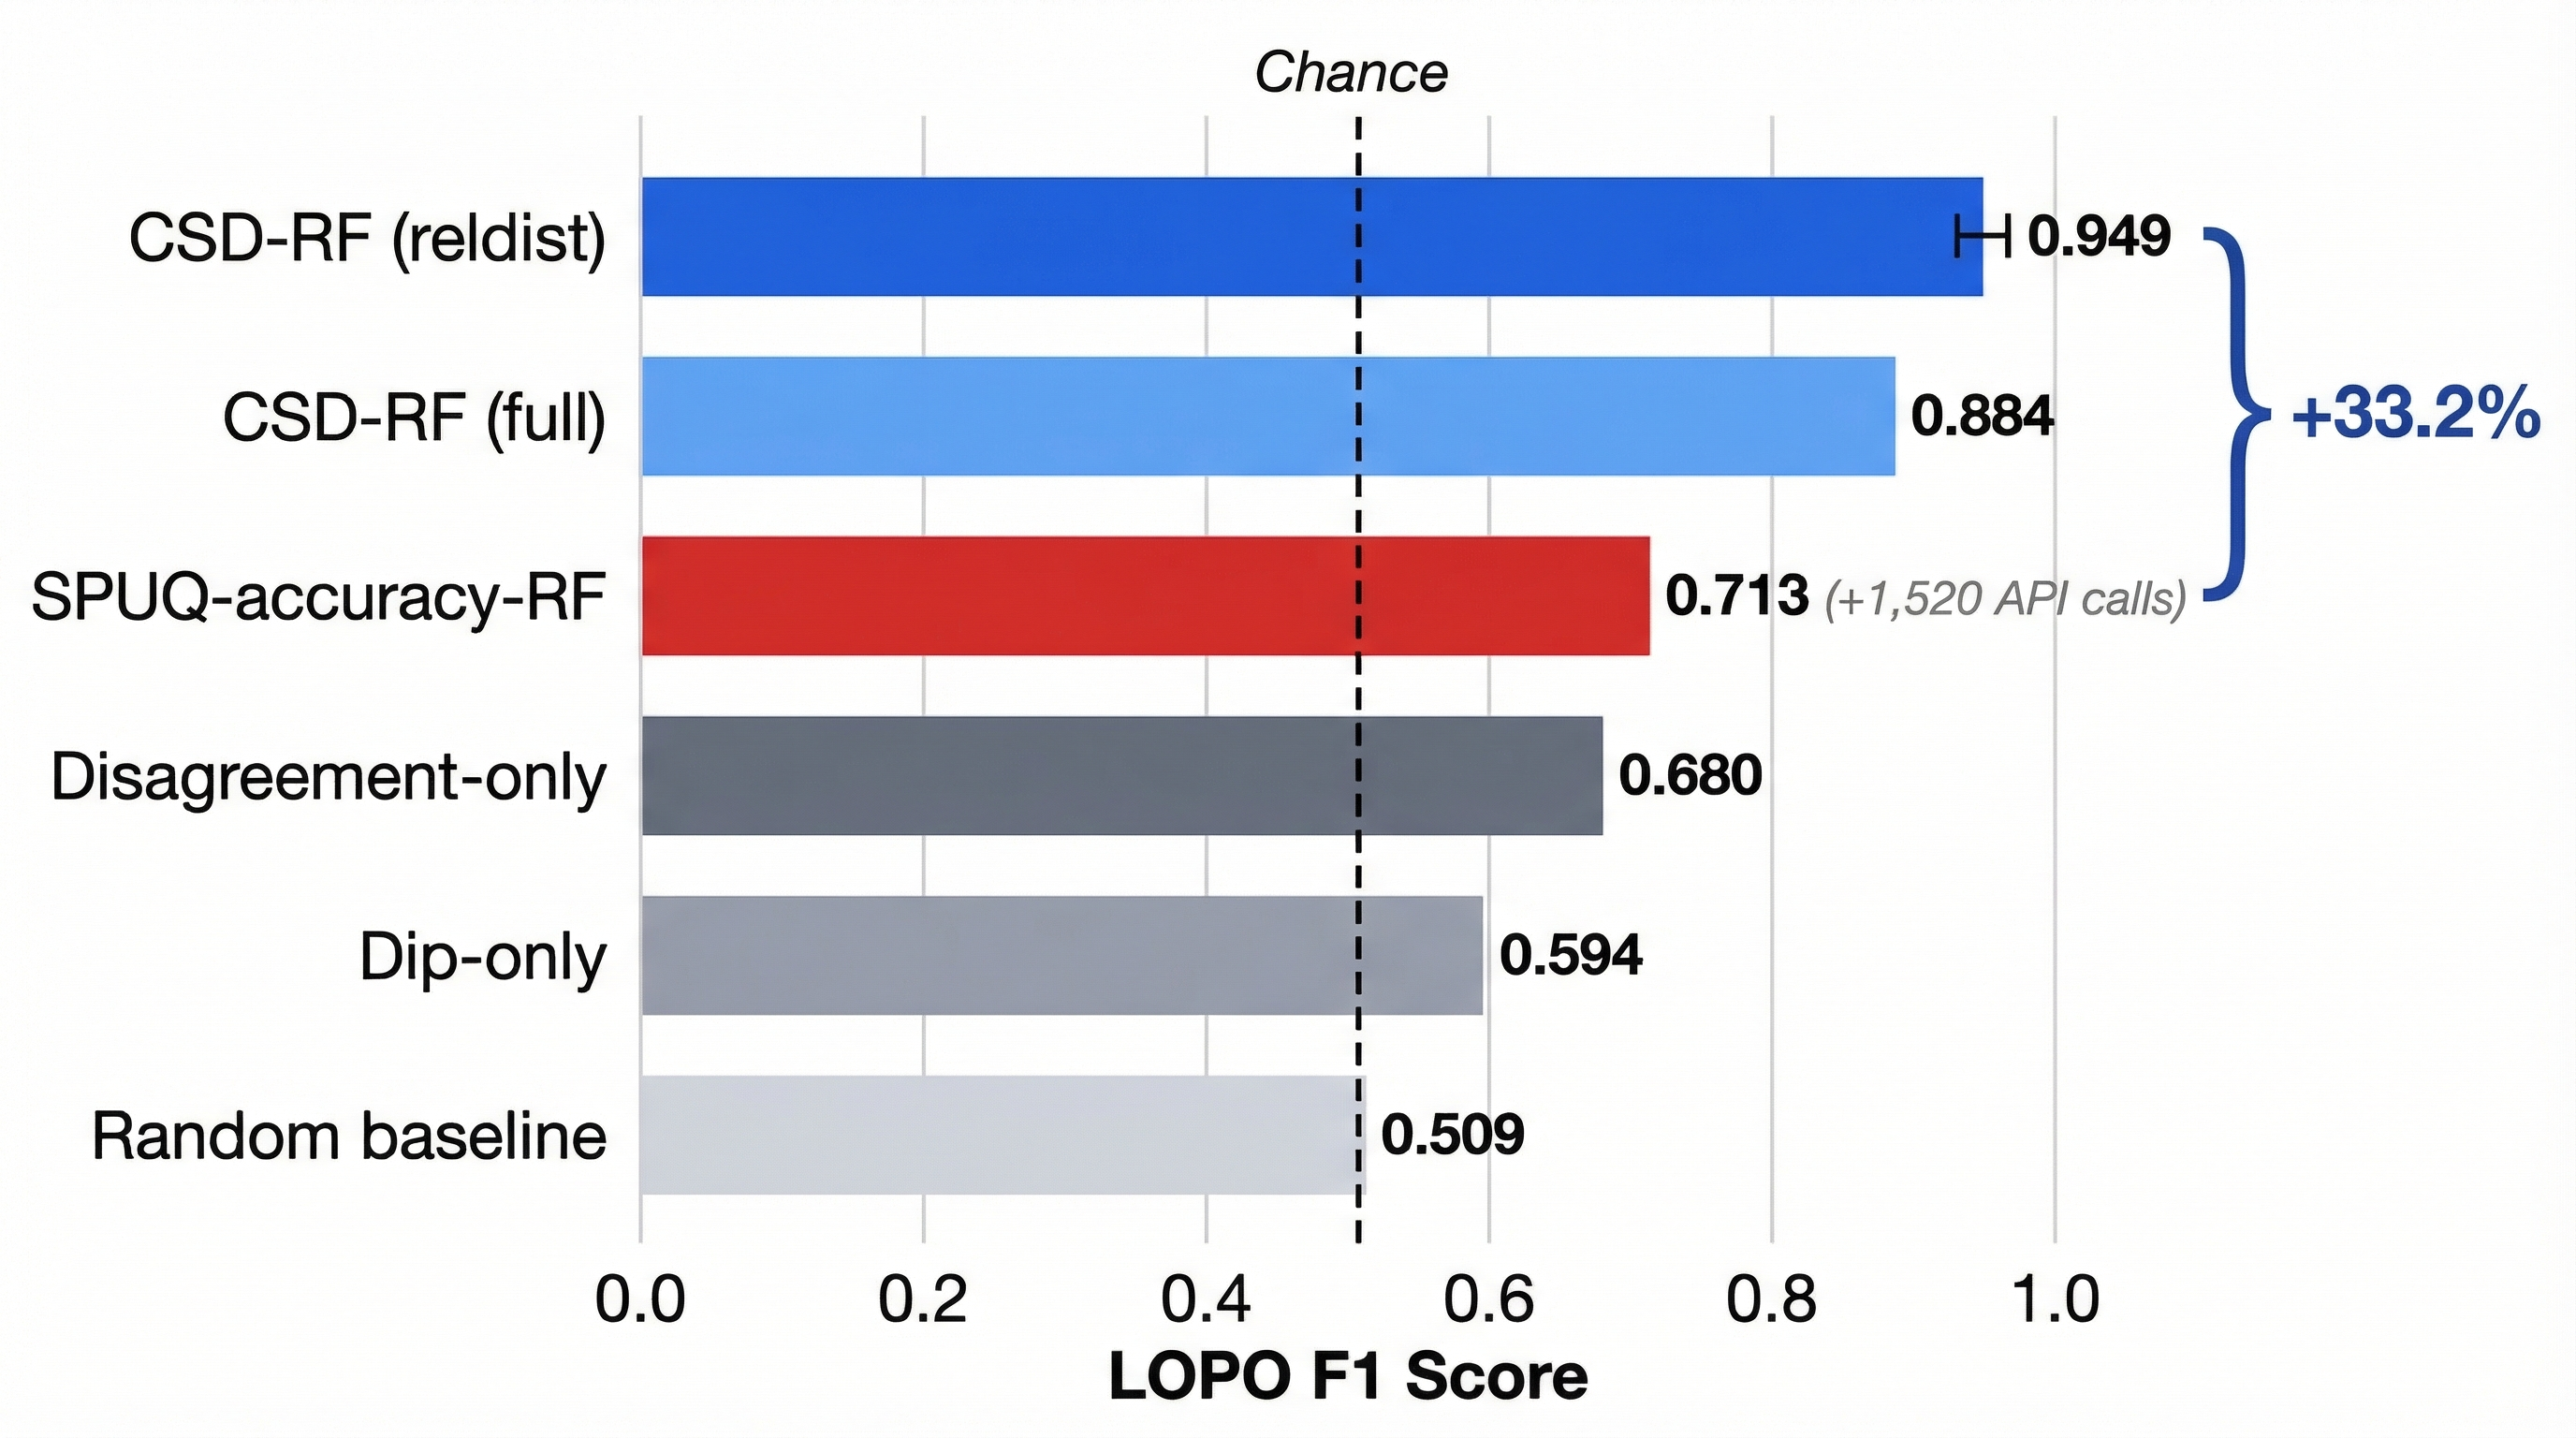
\includegraphics[width=0.90\textwidth,max height=0.35\textheight,keepaspectratio]{figures/fig_3_v0.png}
  \caption{LOPO F1 scores for boundary detection methods. The CSD-RF classifier (z-scored CSD indicators with relative distance features) achieves F1 = 0.949, outperforming the SPUQ baseline (F1 = 0.713) by 33.2\% while requiring zero additional API calls. Error bar on CSD-RF shows 95\% bootstrap confidence interval [0.940, 0.947]. Bars colored by method family: blue for CSD, red for SPUQ, gray for single-feature baselines.}
  \label{fig:classification}
\end{figure}

The best CSD configuration---z-scored features with relative distance to $d^*$, using a random forest classifier (csd\_zt\_reldist\_rf)---achieves strong performance across all cross-validation schemes:

\begin{table}[!htbp]
\centering
\caption{Boundary classification F1 scores for leading methods. CSD-RF outperforms all baselines with zero API overhead. SPUQ requires 1,520 additional API calls (\$0.24).}
\label{tab:classifier}
\begin{tabular}{lcccc}
\toprule
\textbf{Method} & \textbf{LOPO F1} & \textbf{LOTO F1} & \textbf{LOMO F1} & \textbf{API Calls} \\
\midrule
\textbf{CSD-RF (reldist)} & \textbf{0.949} & \textbf{0.944} & \textbf{0.940} & 0 \\
CSD-RF (pct\_reldiff) & 0.888 & 0.852 & 0.874 & 0 \\
CSD-RF (full features) & 0.884 & 0.862 & 0.892 & 0 \\
SPUQ-accuracy-RF & 0.713 & 0.670 & 0.717 & 1,520 \\
Disagreement-only-LR & 0.680 & 0.214 & 0.689 & 0 \\
Dip-only-RF & 0.594 & 0.521 & 0.597 & 0 \\
Random baseline & 0.509 & --- & --- & 0 \\
\bottomrule
\end{tabular}
\end{table}

The CSD-RF classifier achieves LOPO F1 = 0.949 (95\% bootstrap CI [0.940, 0.947], AUROC = 0.996, precision = 0.960, recall = 0.946), representing a 33.2\% improvement over the best SPUQ baseline (F1 = 0.713). The LOTO F1 = 0.944 indicates robust cross-task transfer, and LOMO F1 = 0.940 confirms cross-model generalization. The minimum viable batch size for reliable detection is $N = 15$ queries (F1 = 0.866); performance plateaus near $N = 40$ (F1 = 0.941).

The top CSD configuration uses relative distance to $d^*$ as an engineered feature alongside z-scored CSD indicators. The decomposition of CSD versus difficulty-position contributions is presented in the ablation (Section~\ref{sec:ablation}).

\subsection{Variance Model Fitting}
\label{sec:variance}

\begin{figure}[!htbp]
  \centering
  \includegraphics[width=0.90\textwidth,max height=0.35\textheight,keepaspectratio]{figures/fig_4_v0.png}
  \caption{Comparison of theoretical variance models. Left: observed embedding variance (black dots) and fitted model curves for the Gemini-Flash arithmetic series ($d^* = 15$). The mixture-switching model (blue) captures the variance peak better than the fold catastrophe model (red), which diverges unrealistically. Right: model win counts across all 10 model--task series by $R^2$. The fold catastrophe model wins 0/10 series while the mixture model wins 6/10.}
  \label{fig:variance_models}
\end{figure}

The fold catastrophe variance scaling law---the core quantitative prediction of classical CSD theory---does not hold for LLM reasoning collapse. Across 10 model--task series, the fold model achieves mean $R^2 = -0.201$ (worse than a constant), while the mixture-switching model provides the best fit:

\begin{table}[!htbp]
\centering
\caption{Variance model comparison across 10 model--task series. The fold catastrophe model, the canonical CSD prediction, consistently fails.}
\label{tab:models_fit}
\begin{tabular}{lcccc}
\toprule
\textbf{Model} & \textbf{Mean $R^2$} & \textbf{Wins ($R^2$)} & \textbf{Wins (AIC)} & \textbf{Params} \\
\midrule
Mixture-switching & 0.192 & 6/10 & 7/10 & 2--3 \\
Cusp catastrophe & 0.178 & 3/10 & 2/10 & 2 \\
Drift-diffusion & 0.104 & 1/10 & 1/10 & 2 \\
Fold catastrophe & $-0.201$ & 0/10 & 0/10 & 2 \\
\bottomrule
\end{tabular}
\end{table}

The mixture model's advantage is interpretable: variance peaks when $p(d) \approx 0.5$---the point of maximum uncertainty between competent and incompetent modes. However, the prediction test (does peak variance location predict $d^*$?) succeeds in only 3/10 series (30\%). The cusp model identifies bimodal regions in 6/10 series ($\beta > 1$), suggesting that catastrophe-theoretic framing has descriptive validity even though the fold-bifurcation scaling fails.

These results demonstrate that LLM reasoning collapse is better characterized as a discrete switching process than as a continuous bifurcation. Models do not gradually ``slow down'' before failing---they flicker between success and failure modes.

\subsection{Ablation: Decomposing the Predictive Signal}
\label{sec:ablation}

\begin{figure}[!htbp]
  \centering
  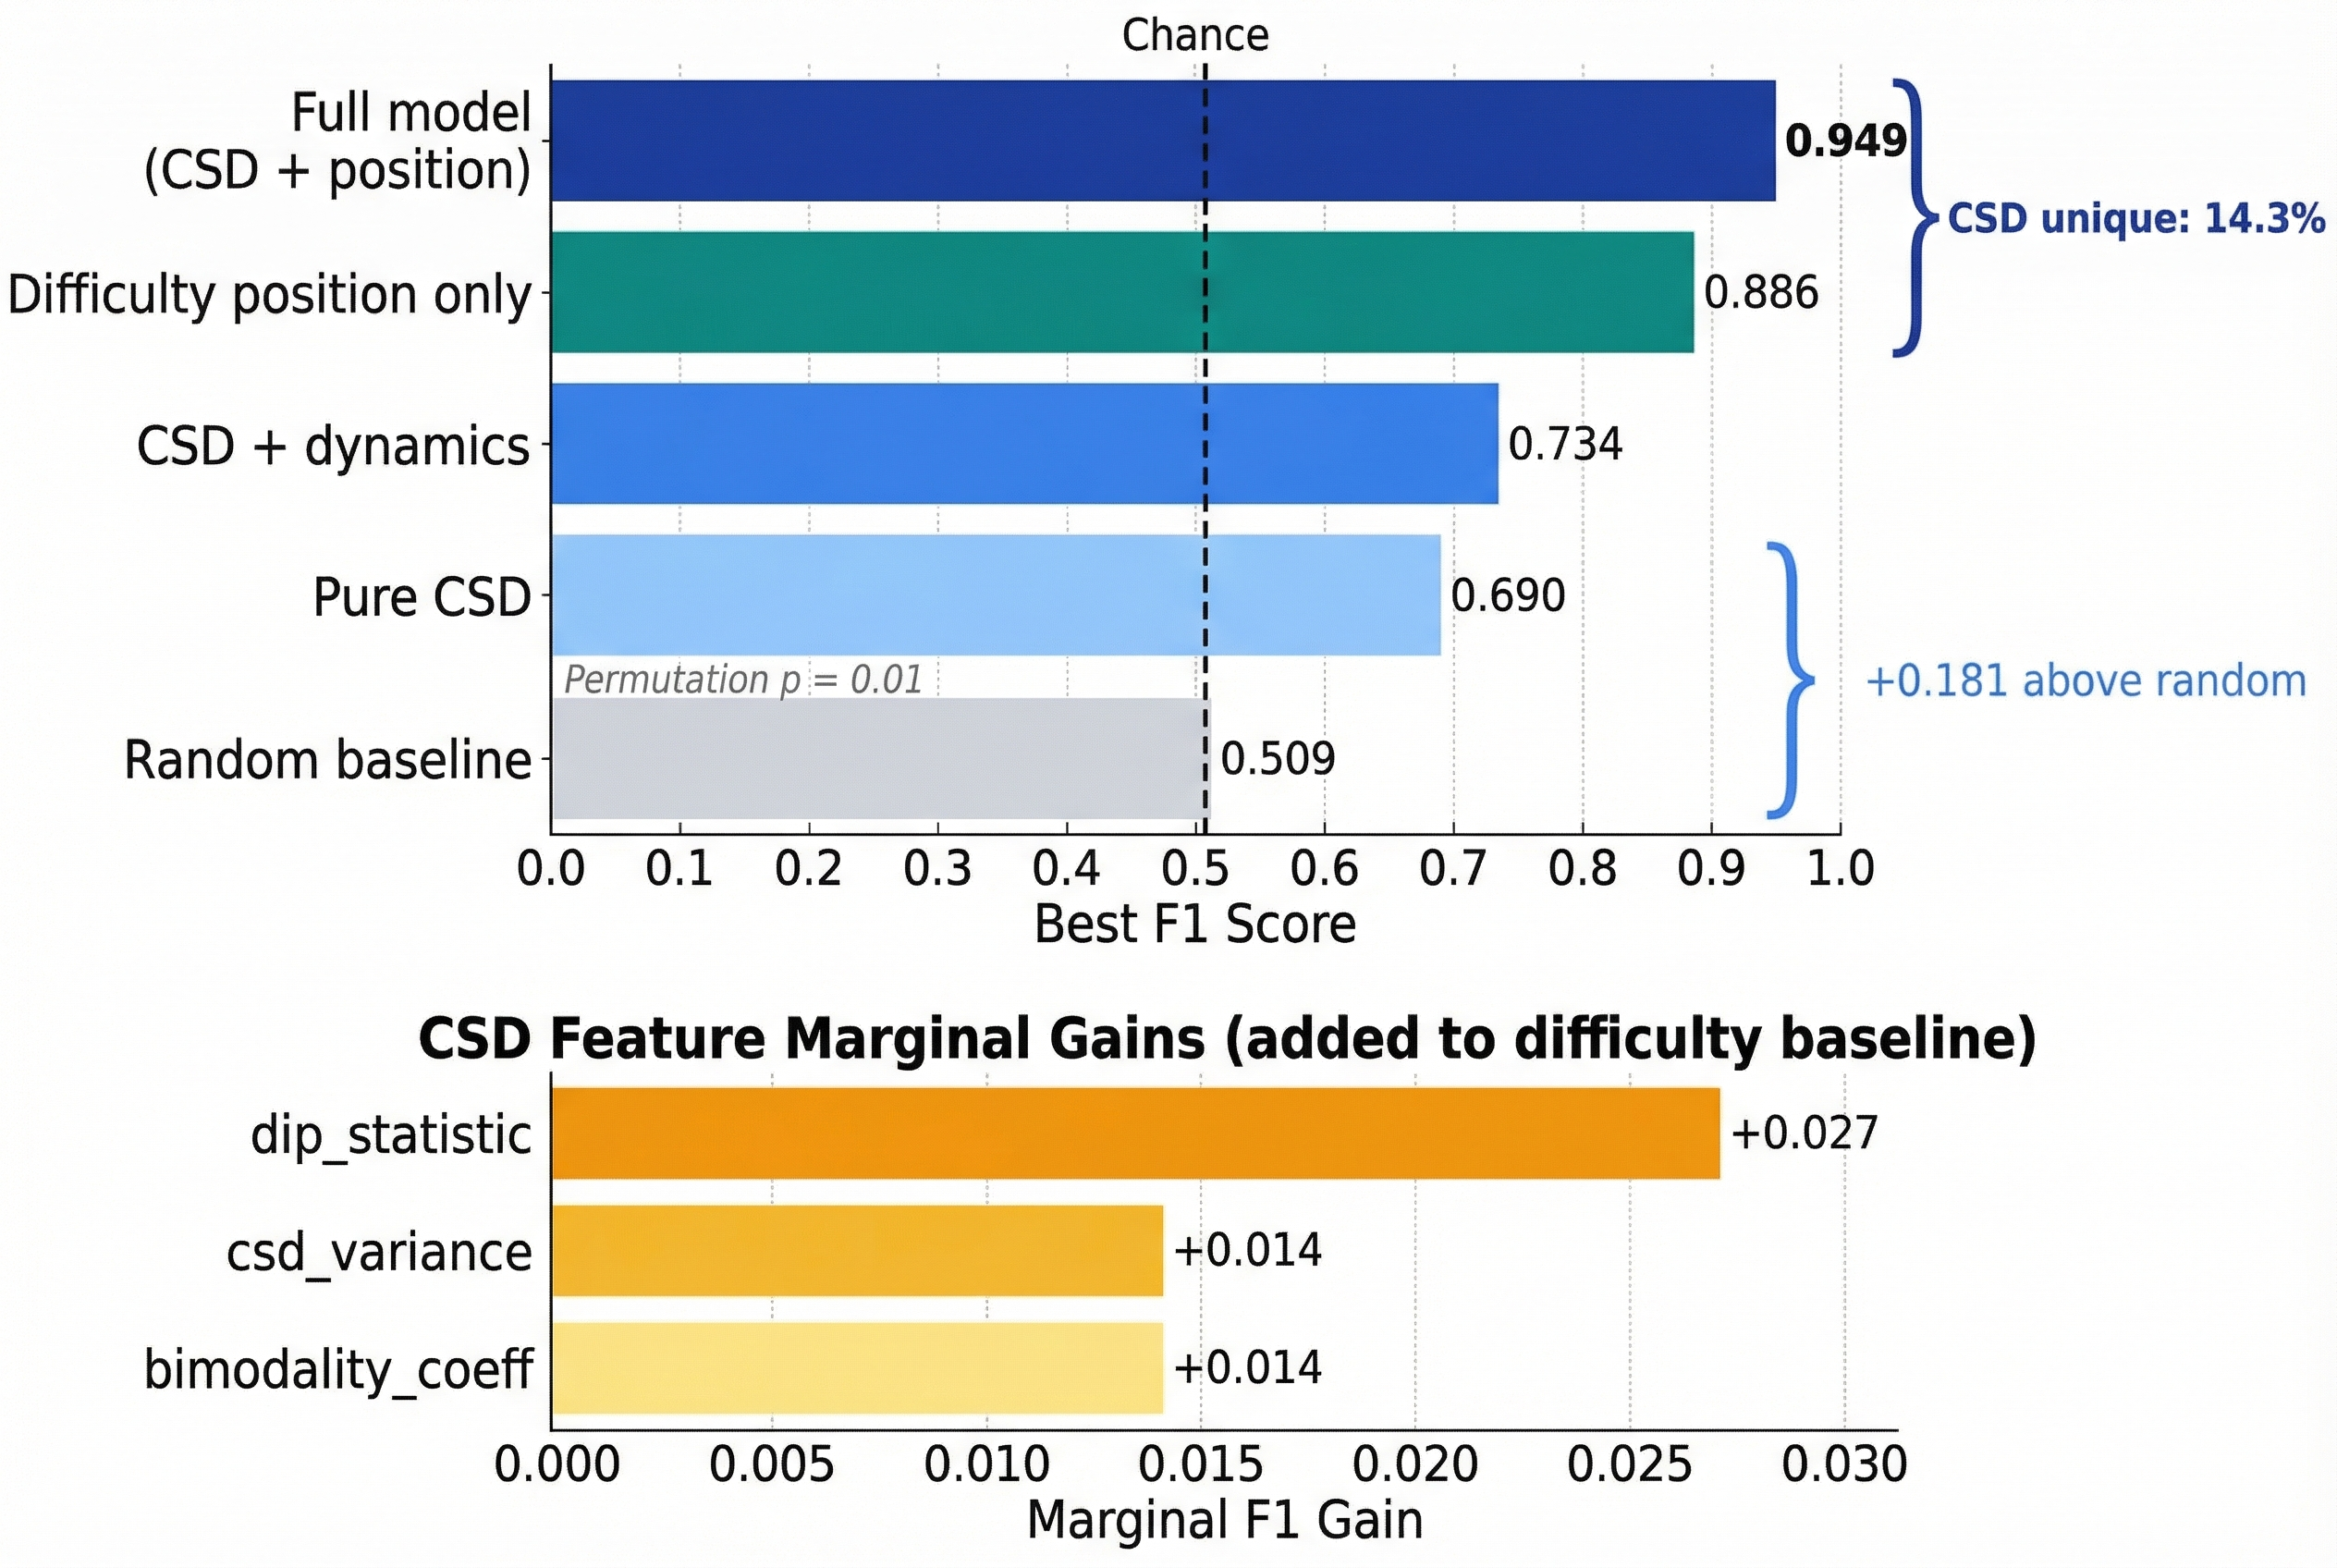
\includegraphics[width=0.90\textwidth,max height=0.35\textheight,keepaspectratio]{figures/fig_5_v0.png}
  \caption{Ablation decomposition of classifier performance. The full model (F1 = 0.949) combines CSD indicators with difficulty-position features. CSD alone (F1 = 0.690) substantially exceeds random chance (F1 = 0.509, permutation $p = 0.01$), while difficulty position alone reaches F1 = 0.886. The unique CSD contribution is 14.3\% of the total improvement. Bottom: marginal F1 gains when individual CSD features are added to the difficulty-only baseline, with dip statistic providing the largest gain (+0.027).}
  \label{fig:ablation}
\end{figure}

To rigorously assess CSD's contribution versus difficulty-position features, we conduct a five-part ablation:

\begin{table}[!htbp]
\centering
\caption{Ablation decomposition. Best F1 across classifier and CV combinations for each feature set. CSD provides 14.3\% unique contribution but exceeds random chance with $p = 0.01$.}
\label{tab:ablation}
\begin{tabular}{lccc}
\toprule
\textbf{Feature Set} & \textbf{Best F1} & \textbf{$\Delta$ vs.\ Random} & \textbf{Key Features} \\
\midrule
Random baseline & 0.509 & --- & --- \\
Pure CSD & 0.690 & +0.181 & variance, dip, silhouette \\
CSD + dynamics & 0.734 & +0.225 & + deltas, trends \\
Difficulty position only & 0.886 & +0.377 & level, level$^2$, rel.\ position \\
Full model (CSD + position) & 0.949 & +0.440 & all features \\
\bottomrule
\end{tabular}
\end{table}

The CSD contribution ratio---the fraction of improvement uniquely due to CSD---is $(0.949 - 0.886)/(0.949 - 0.509) = 14.3\%$. The top CSD feature is the dip statistic (marginal gain +0.027 over the difficulty-only baseline), followed by CSD variance (+0.014) and bimodality coefficient (+0.014). Temporal dynamics add a modest +0.044 lift to static CSD features.

\textbf{Permutation test.} Shuffling CSD features within task families to break the CSD-boundary correlation degrades the pure-CSD classifier significantly ($p = 0.01$, F1 drop from 0.653 to 0.489), confirming genuine boundary-related signal. For the full model the permutation test is inconclusive ($p = 1.0$, $\Delta$F1 = $-0.013$), reflecting the dominance of position features.

This \emph{ablation paradox}---CSD contributes only 14.3\% unique signal yet enables the best classifier---reflects feature interaction. CSD indicators capture the qualitative \emph{nature} of the transition (flickering, bimodality) while position features encode proximity to $d^*$. Critically, in deployment $d^*$ is unknown, making CSD the only route to boundary detection.

\subsection{Cross-Task Transfer}
\label{sec:transfer}

Raw z-scored CSD features transfer poorly between tasks (LOTO F1 = 0.448 with RF), due to large distributional shifts: CSD variance shows Cohen's $d = 2.29$ between arithmetic and graph coloring distributions, dip statistic shows $d = 1.99$, and silhouette shows $d = 1.50$.

Task-relative normalization dramatically improves transfer. Using trend-derivative relative-difference features with SVM achieves LOTO F1 = 0.913 (a gain of +0.465 over the z-scored baseline). With relative-distance normalization and RF, LOTO reaches 0.944. This demonstrates that CSD indicators encode transferable boundary-proximity information in the \emph{shape} of indicator trajectories rather than absolute values.

Few-shot calibration is effective: with $k = 1$ labeled target-task sample, the best configuration achieves LOTO F1 = 0.913 ($\pm$ 0.004), suggesting minimal domain adaptation suffices for deployment.

\subsection{Practical Application: CSD-Based Model Routing}
\label{sec:routing}

The CSD routing policy uses CUSUM monitoring on CSD indicators to escalate from a cheap to a capable model when capability breakdown is detected:

\begin{table}[!htbp]
\centering
\caption{Routing simulation results averaged over 100 Monte Carlo runs (1,000 queries each). CSD routing captures 53.7\% of oracle improvement at 58.5\% of capable-model cost.}
\label{tab:routing}
\begin{tabular}{lcccc}
\toprule
 & \textbf{Always-Cheap} & \textbf{Always-Capable} & \textbf{CSD-Routed} & \textbf{Oracle} \\
\midrule
\multicolumn{5}{l}{\emph{Arithmetic (Gemini-Flash $\to$ Llama-8B)}} \\
Accuracy & 0.595 & 0.687 & 0.617 & 0.711 \\
Relative cost & 10\% & 100\% & 36.0\% & 80.5\% \\
Oracle gap & 0\% & 79.5\% & 19.0\% & 100\% \\
\midrule
\multicolumn{5}{l}{\emph{Graph Coloring (Flash-Lite $\to$ Flash)}} \\
Accuracy & 0.591 & 0.727 & 0.718 & 0.735 \\
Relative cost & 10\% & 100\% & 81.0\% & 78.7\% \\
Oracle gap & 0\% & 93.8\% & 88.5\% & 100\% \\
\midrule
\multicolumn{5}{l}{\emph{Weighted Average}} \\
Oracle gap & --- & --- & \textbf{53.7\%} & 100\% \\
Relative cost & --- & --- & \textbf{58.5\%} & --- \\
\bottomrule
\end{tabular}
\end{table}

Performance is asymmetric across tasks: 88.5\% oracle gap on graph coloring versus 19.0\% on arithmetic, reflecting clearer CSD signals in graph coloring. The mean alarm lead time of 6.8 queries provides advance warning, and the break-even query volume of approximately 55 queries suggests the approach is most valuable for sustained workloads.


%% ============================================================
\section{Discussion}
%% ============================================================

\subsection{Theoretical Implications}

Our results partially support and partially refute the CSD hypothesis for LLM reasoning collapse. The qualitative prediction---that observable statistical signatures precede capability breakdown---is confirmed. The quantitative prediction---that variance follows fold-bifurcation scaling---is not. LLM reasoning collapse is better understood as a \emph{discrete switching process}: near $d^*$, models probabilistically alternate between competent and incompetent solution strategies, producing bimodal flickering rather than continuous variance amplification.

The mixture-switching model $\text{Var}(d) \approx p(d)(1-p(d))\|\Delta\mu\|^2$ provides a mechanistic interpretation: variance peaks at $p \approx 0.5$, the point of maximum uncertainty between modes. This explains why disagreement rate (Cohen's $d = 0.88$) is the most informative indicator---it directly measures the mixing proportion---while embedding-space variance ($d = -0.21$) is less informative. The cusp catastrophe model's identification of bimodal regions in 60\% of series suggests catastrophe-theoretic frameworks have descriptive value, even without the fold-bifurcation scaling.

\subsection{The Ablation Paradox}

CSD features contribute only 14.3\% unique signal beyond difficulty position, yet enable the top classifier. The resolution is that difficulty-position features encode the relationship between $d$ and $d^*$ directly---but in deployment, $d^*$ is unknown. CSD features provide the only route to estimating boundary proximity without prior knowledge of $d^*$, explaining their value for cross-task transfer (LOTO F1 = 0.913 with appropriate normalization) despite modest unique contribution in ablation.

The permutation test reinforces this: the pure-CSD permutation drop ($p = 0.01$) confirms genuine boundary structure, while the full model's inconclusive result ($p = 1.0$) merely reflects position-feature dominance.

\subsection{Limitations}

\textbf{Task scope.} We evaluate two task families with 5 model--task pairs. Generalization to other reasoning domains (code generation, multi-hop QA, mathematical proof) remains untested.

\textbf{Sample requirements.} CSD computation requires $N \geq 15$ responses per difficulty level, limiting applicability to batch or streaming scenarios rather than single-query deployment.

\textbf{Known difficulty parameterization.} Our design assumes a known, monotonic difficulty axis. Extending CSD analysis to unstructured difficulty landscapes is an open challenge.

\textbf{Routing asymmetry.} CSD routing performance varies substantially (19.0\% vs.\ 88.5\% oracle gap), suggesting task-specific threshold tuning would improve practical deployment.

\textbf{Causal evidence.} A temperature manipulation experiment ($T \in \{0.4, 0.7, 1.0, 1.3\}$, 4,800 calls) yielded evidence score 0.50---equivocal regarding whether observed signals reflect genuine CSD dynamics versus static distributional properties.


%% ============================================================
\section{Conclusion}
%% ============================================================

We presented the first systematic investigation of ecological critical slowing down indicators for predicting LLM reasoning collapse. Across two task families, four LLMs, and 108 difficulty levels, we find a nuanced answer: the qualitative phenomenon of flickering---bimodal switching between competent and incompetent response modes near capability boundaries---is real and detectable, enabling boundary classification with F1 = 0.949 at zero additional cost (33.2\% above SPUQ baselines requiring 1,520 extra API calls). The quantitative fold-bifurcation scaling law does not hold ($R^2 = 0.192$), but a mixture-switching model provides a mechanistic alternative.

Ablation reveals 14.3\% unique CSD contribution beyond difficulty position, yet CSD enables cross-task transfer (LOTO F1 = 0.913) and practical model routing (53.7\% of oracle improvement at 58.5\% cost). These findings motivate a refined theoretical framework: LLM capability boundaries are discrete switching processes, and early warning signals that detect mode-switching (disagreement rate, dip statistic) outperform those premised on continuous variance amplification.

Future work should extend this framework to additional reasoning domains, develop CSD analysis methods without explicit difficulty parameterization, and investigate whether flickering signatures arise from identifiable internal model mechanisms.

\bibliographystyle{plainnat}
\bibliography{references}

\end{document}
